\renewcommand{\EntradaBibtex}{pr14010164}

\begin{frame}{\citetitle{\EntradaBibtex} \footnotemark[1] (1)}
Problemática: 
\begin{itemize}
    \item Las máquinas industriales de clasificación de fruta utilizan tecnología que lleva muchos años en funcionamiento.
    \item Los algoritmos de clasificación son cerrados y no es posible agregar adecuaciones. 

\end{itemize}
\footnotetext[1]{\fullcite{\EntradaBibtex}}
\end{frame}

\begin{frame}{\citetitle{\EntradaBibtex} (2)}
Propuesta de solución: 
\begin{itemize}
    \item Se desarrolló  un sistema de visión por computadora para clasificar limones por tamaño en tiempo real, integrado directamente en una máquina clasificadora de nivel industrial.
    \item Se evaluaron modelos de aprendizaje automático combinados con análisis de imágenes para estimar las dimensiones (diámetro/tamaño) de los cítricos de forma automática.
    \item Se incorporó un algoritmo de gestión de colas para coordinar el procesamiento de imágenes con el desplazamiento físico de las frutas en la cinta transportadora, garantizando la sincronización precisa entre la detección y los desviadores mecánicos (ejectors).
\end{itemize}

\end{frame}

\begin{frame}{\citetitle{\EntradaBibtex} (3)}
\begin{columns}
\begin{column}{0.45\textwidth}
Materiales:
\begin{itemize}
    \item Una computadora embebida (SBC - Raspberry Pi 4 model B+) 
    \item Una cámara industrial USB 3.0 (HT-SUA134GC-T1V Huateng)
    \item Un microcontrolador Arduino Mega 2560.
    \item Anillo de iluminación led.
    \item Driver para solenoides.                 
\end{itemize}
\end{column}
\begin{column}{0.25\textwidth}
\begin{center}
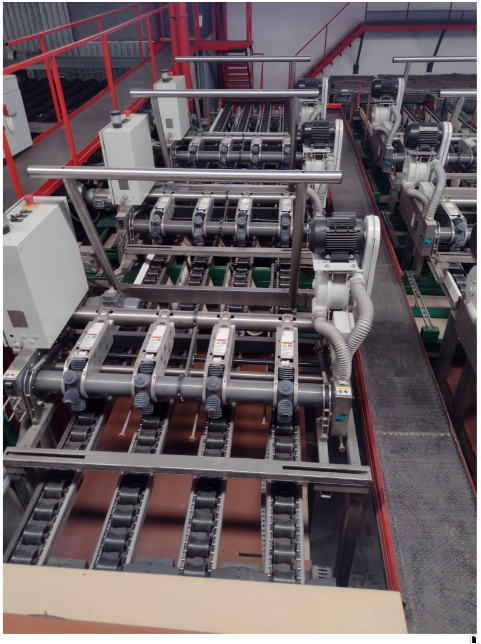
\includegraphics[width=0.90\linewidth]{2026_Citricos/figs/BandaTransportadoraA.png}    
\end{center}   
\end{column}
\begin{column}{0.25\textwidth}
\begin{center}
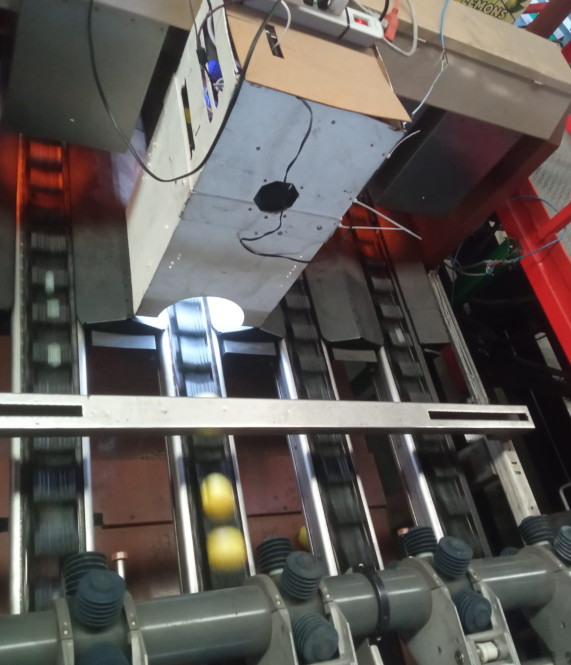
\includegraphics[width=0.90\linewidth]{2026_Citricos/figs/Prototype.jpg}    
\end{center}   
\end{column}

\end{columns}
\end{frame}


\begin{frame}{\citetitle{\EntradaBibtex} (4)}
\begin{center}
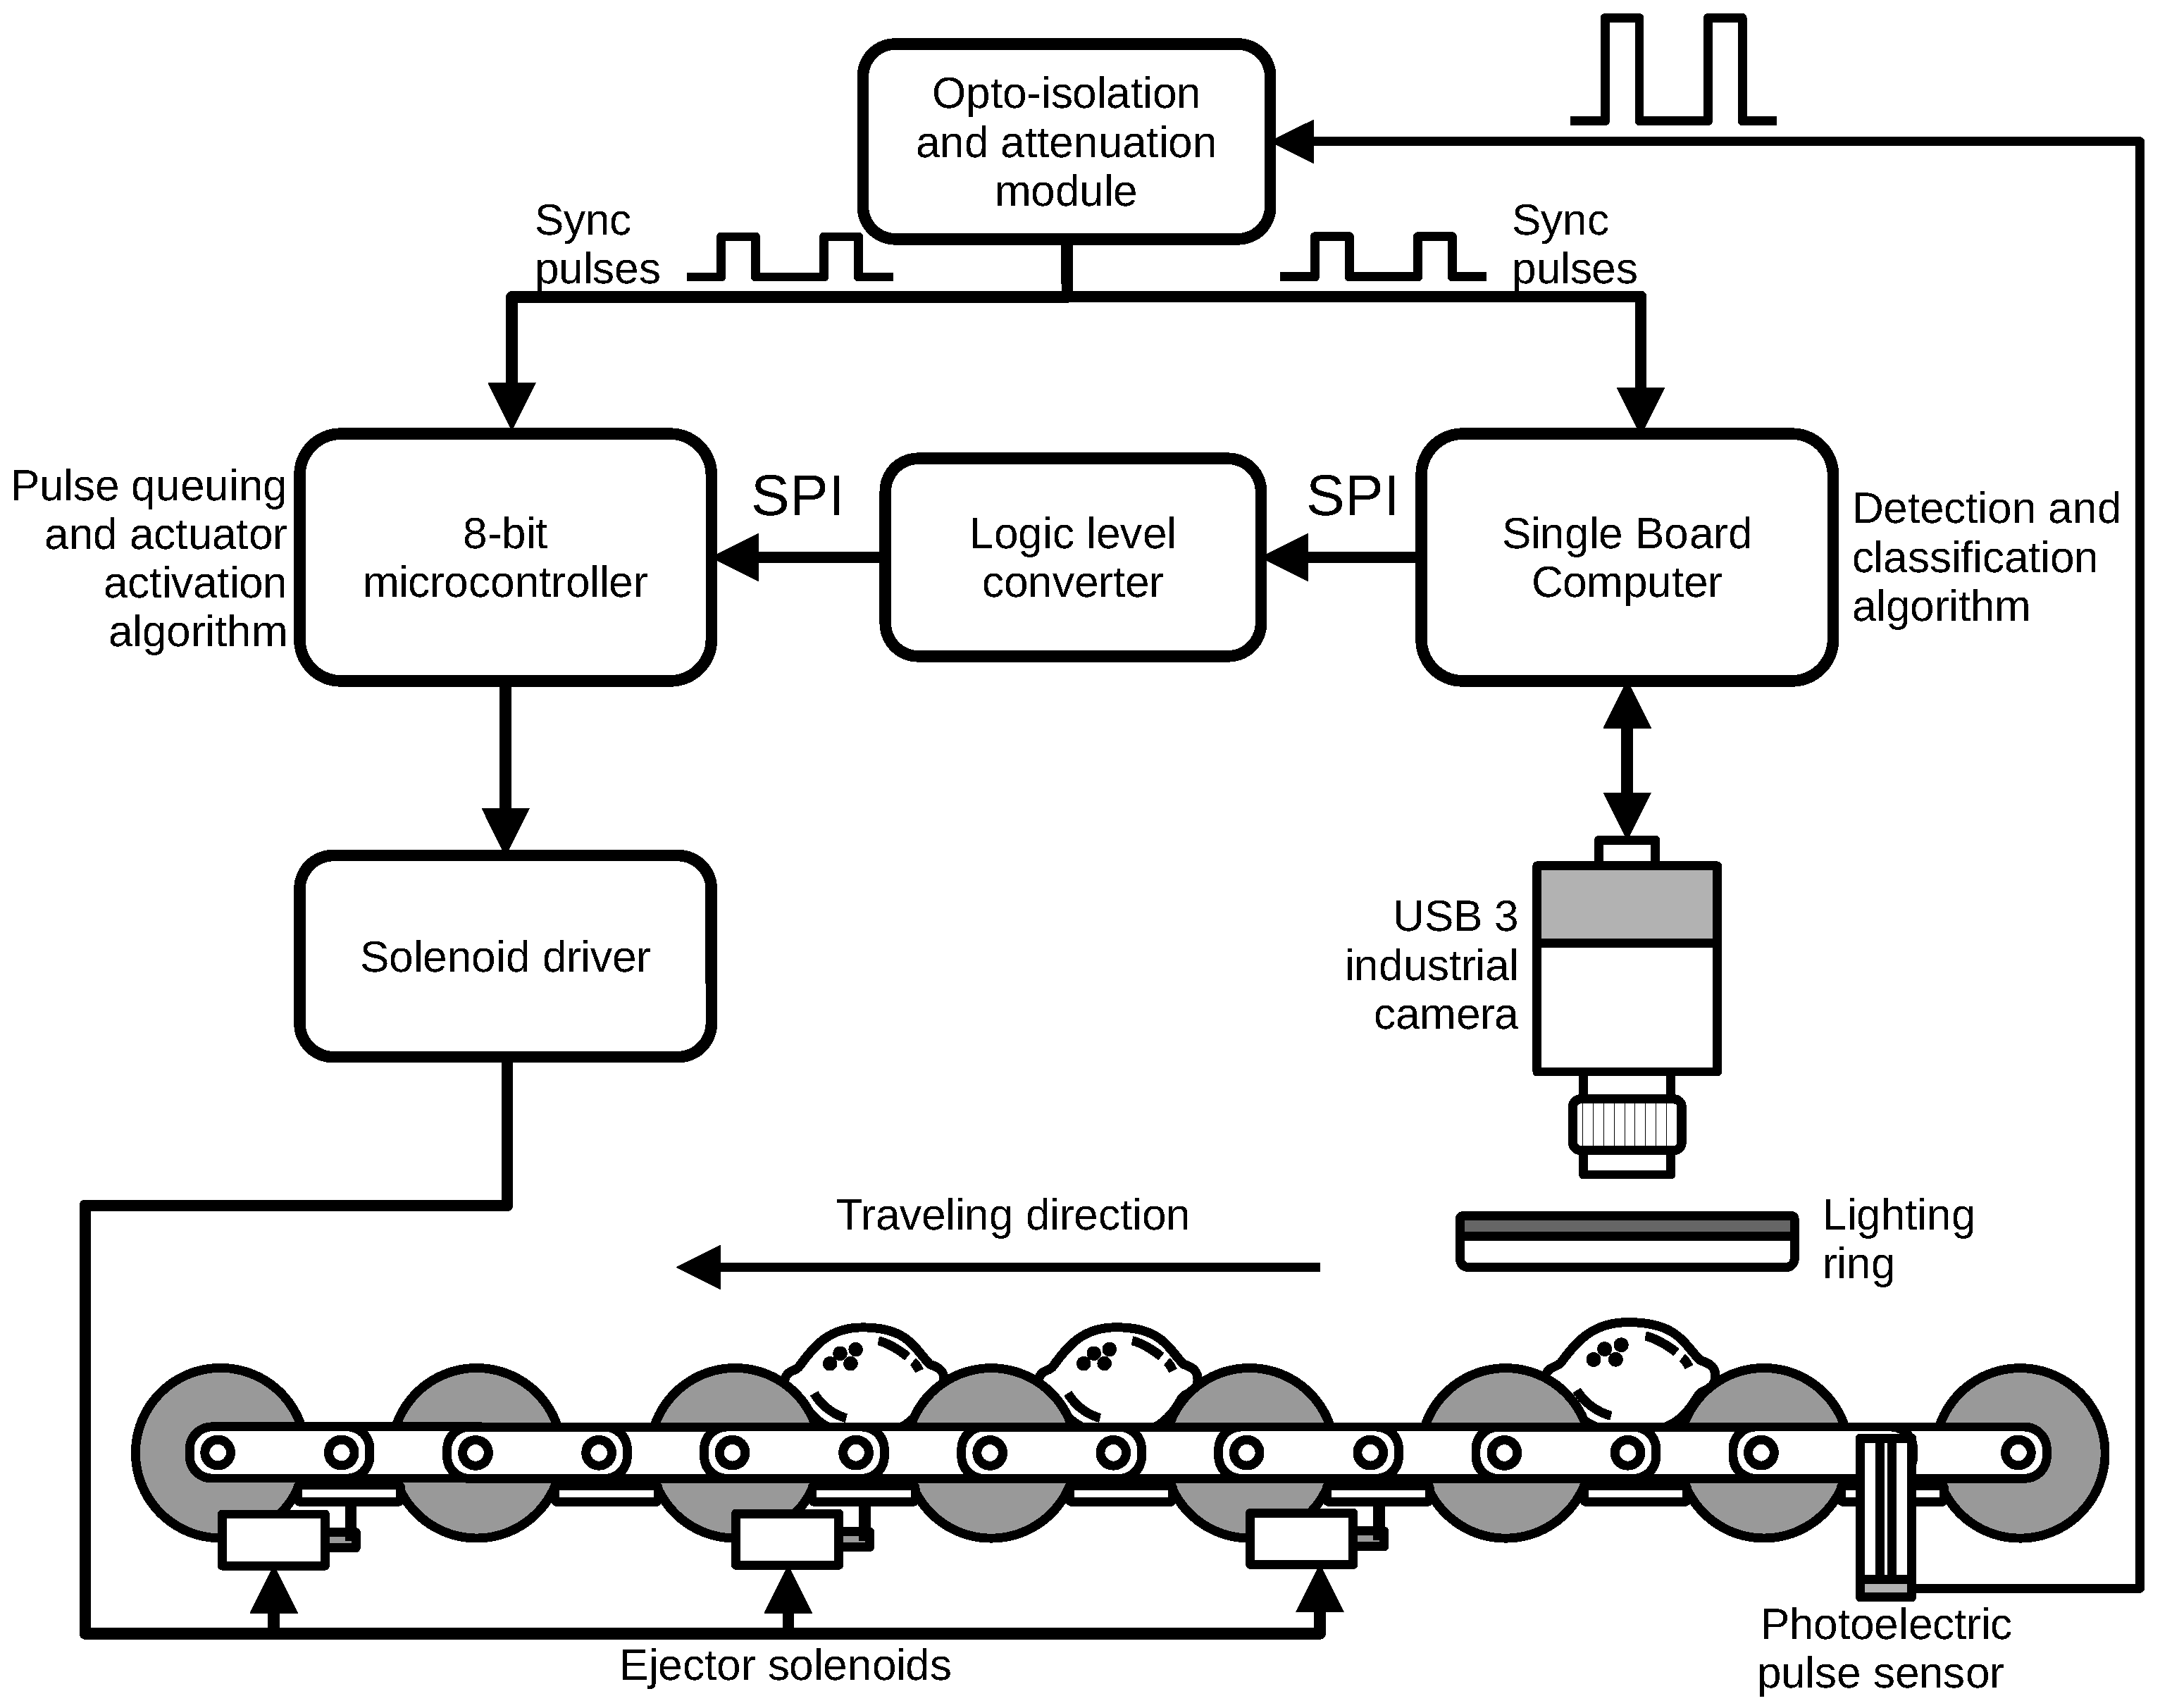
\includegraphics[width=0.50\linewidth]{2026_Citricos/figs/SortingMachine.png}    
\end{center}    
\end{frame}



\begin{frame}{\citetitle{\EntradaBibtex} (5)}
\begin{center}
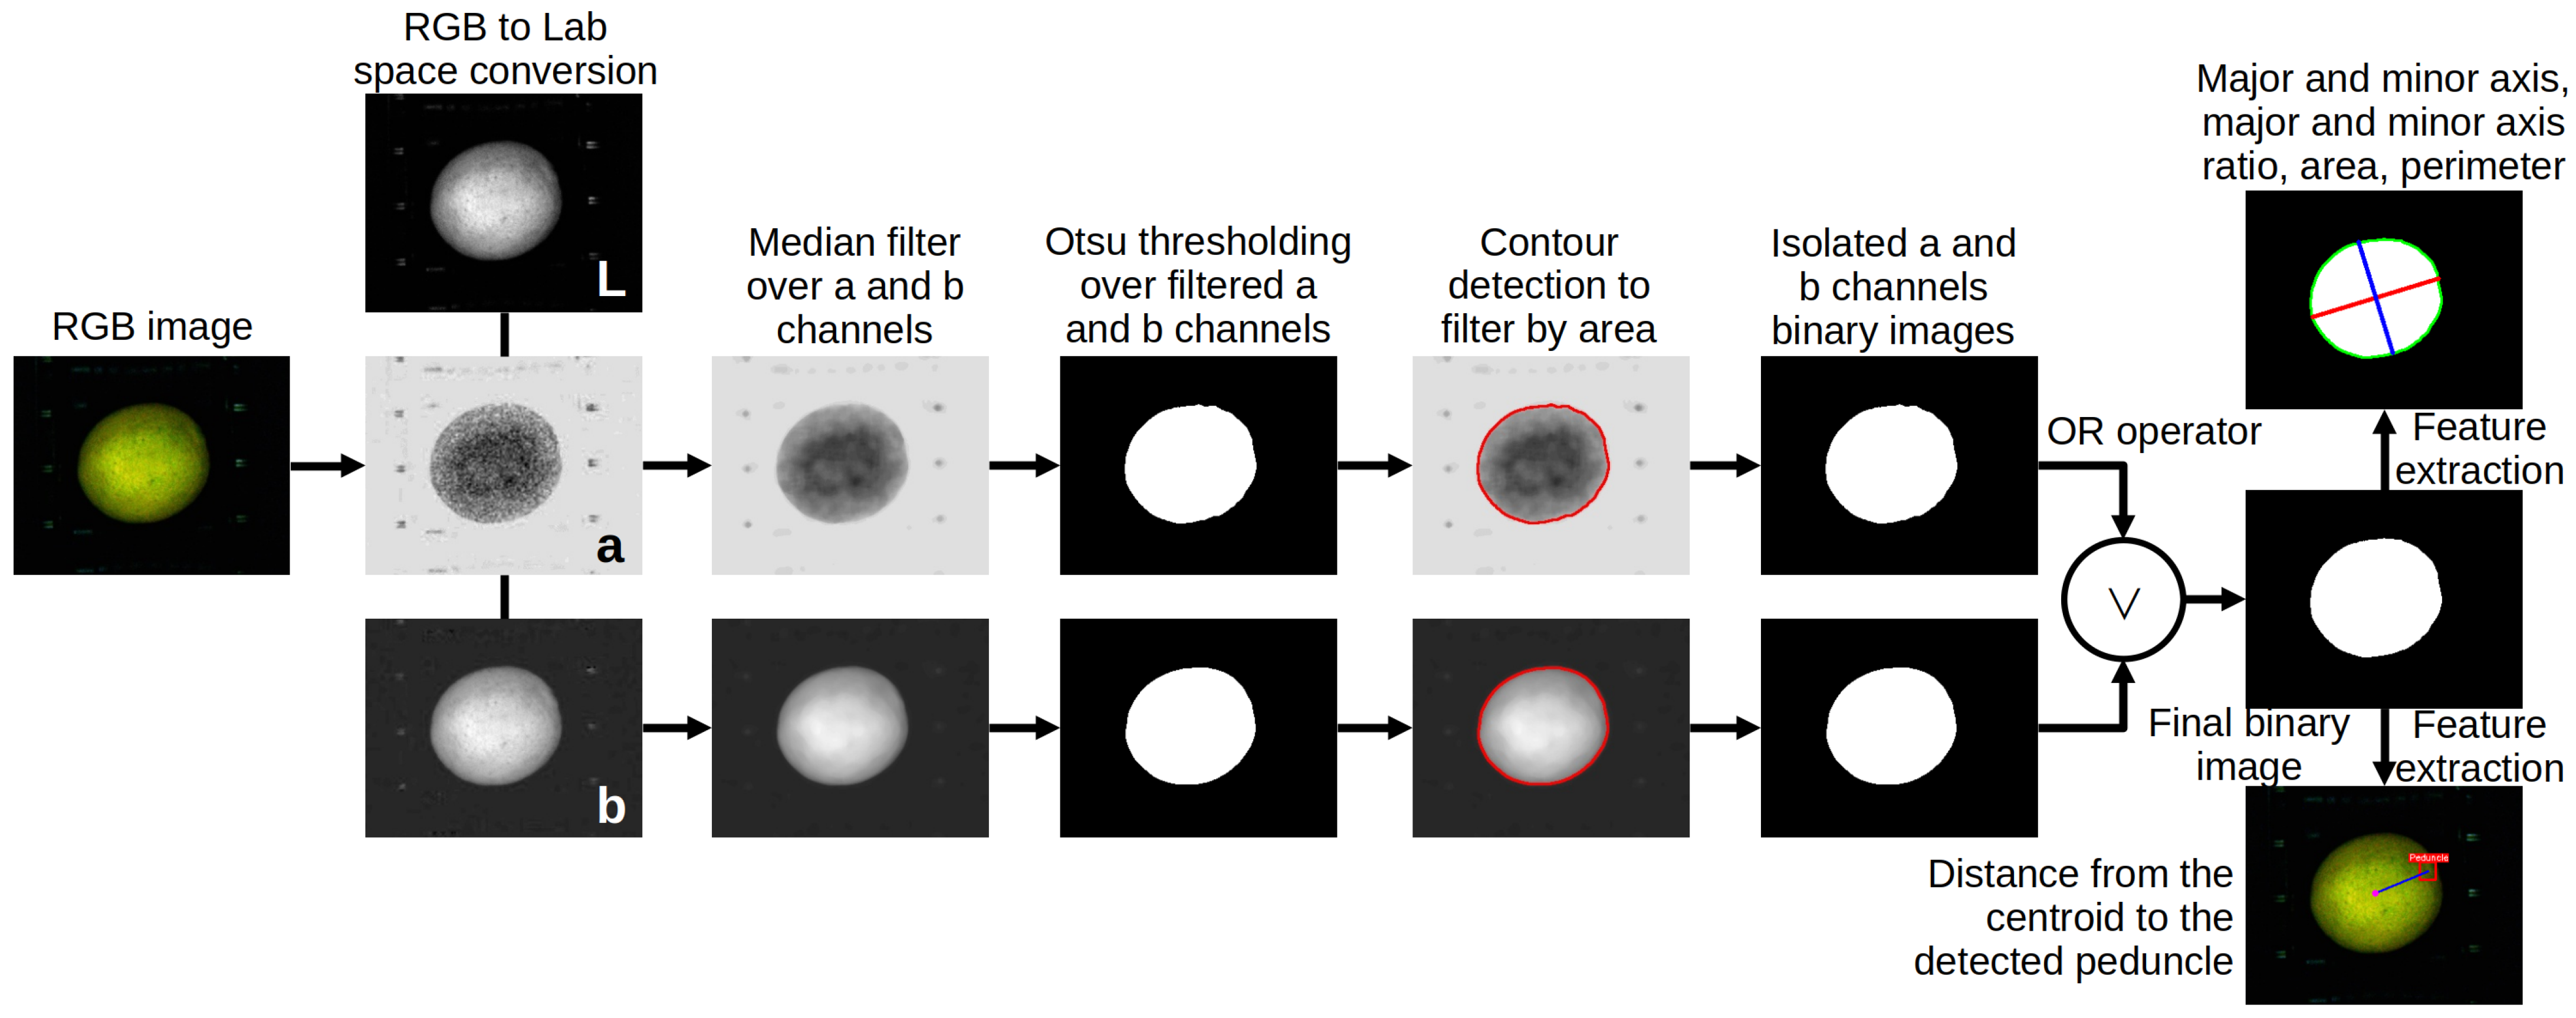
\includegraphics[width=0.92\linewidth]{2026_Citricos/figs/ImageProcessingPipeline_processes-14-00164-g006.png}    
\end{center}    
\end{frame}

\begin{frame}{\citetitle{\EntradaBibtex} (6)}
\begin{columns}
\begin{column}{0.75\textwidth}
Medición del tamaño de los limones: \\
\begin{itemize}
    \item Se utiliza un calibrador mecánico para medir el tamaño de los limones según los estándares de la industria citrícola. 
    \item El dispositivo cuenta con mordazas ajustables que miden el diámetro del eje menor del limón, y que determina el código de tamaño de la fruta (``cantidad''), que indica cuántos limones caben en una caja estándar de 40 libras. Estos tamaños son (75, 95, 115, 140, 165, y 200). 
\end{itemize}
Problema: \\
\begin{itemize}
    \item Los rangos de medición disponibles se superponen, lo que puede generar errores de clasificación, y que esto suele estar sujeto a la interpretación del usuario.
\end{itemize}

\end{column}
\begin{column}{0.25\textwidth}
\begin{center}
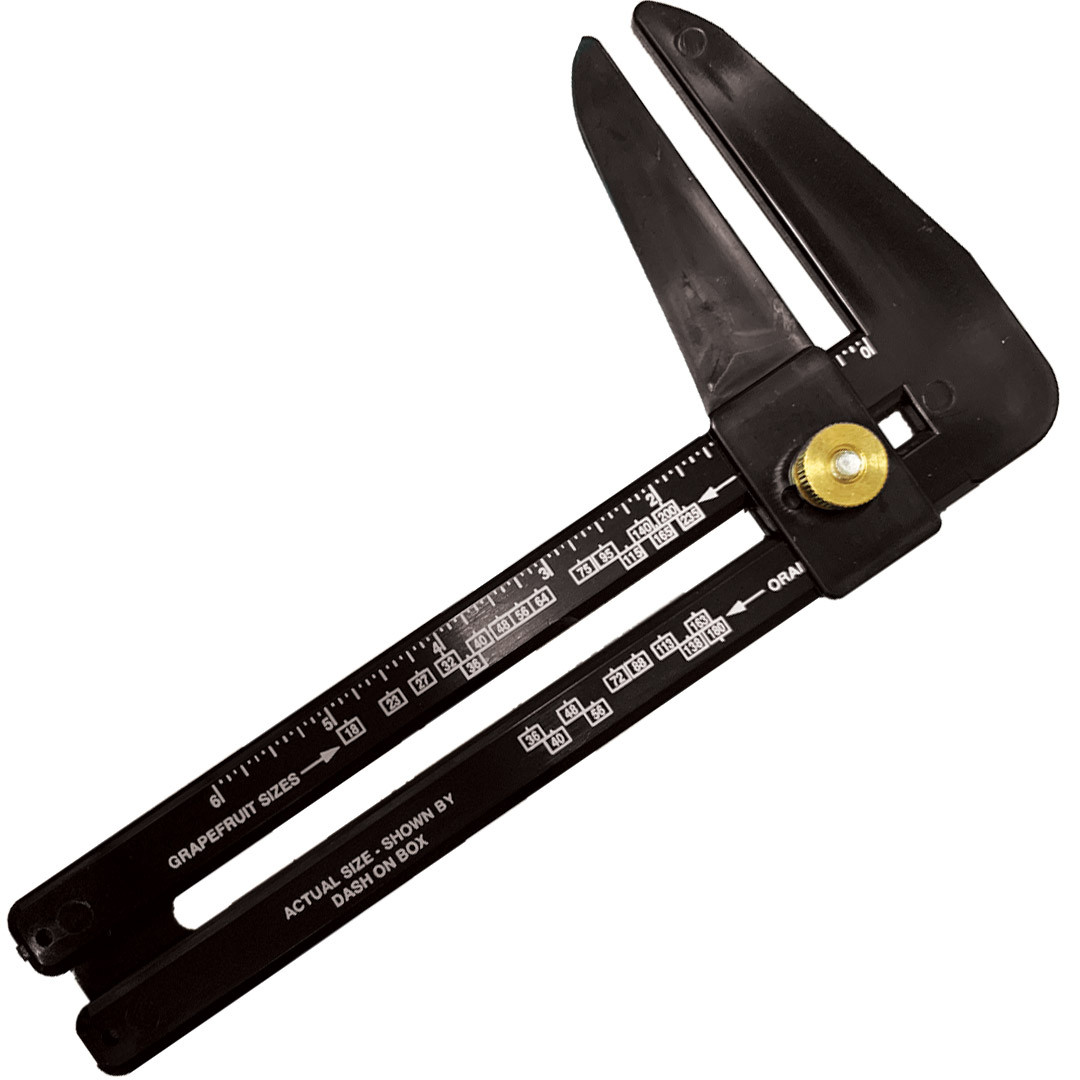
\includegraphics[width=0.95\textwidth]{2026_Citricos/figs/califer.jpg}  
\tiny{\url{https://qasupplies.com/citrus-produce-calipers/}}
\end{center}    
\end{column}
\end{columns}
\end{frame}



\begin{frame}{\citetitle{\EntradaBibtex} (7)}
\begin{columns}
\begin{column}{0.45\textwidth}
Validación del modelo en campo: \\
\begin{itemize}
    \item Se utilizó una muestra de limones independiente al dataset utilizado para entrenar el modelo
    \item Se clasificaron 1,558 limones distribuidos en las siguients clases: 175 (95), 241 (115), 308 (140), 390 (165) y 444 (200). 
    \item Se alcanzó una exactitud del 78\%.
\end{itemize}

\end{column}
\begin{column}{0.45\textwidth}
\begin{center}
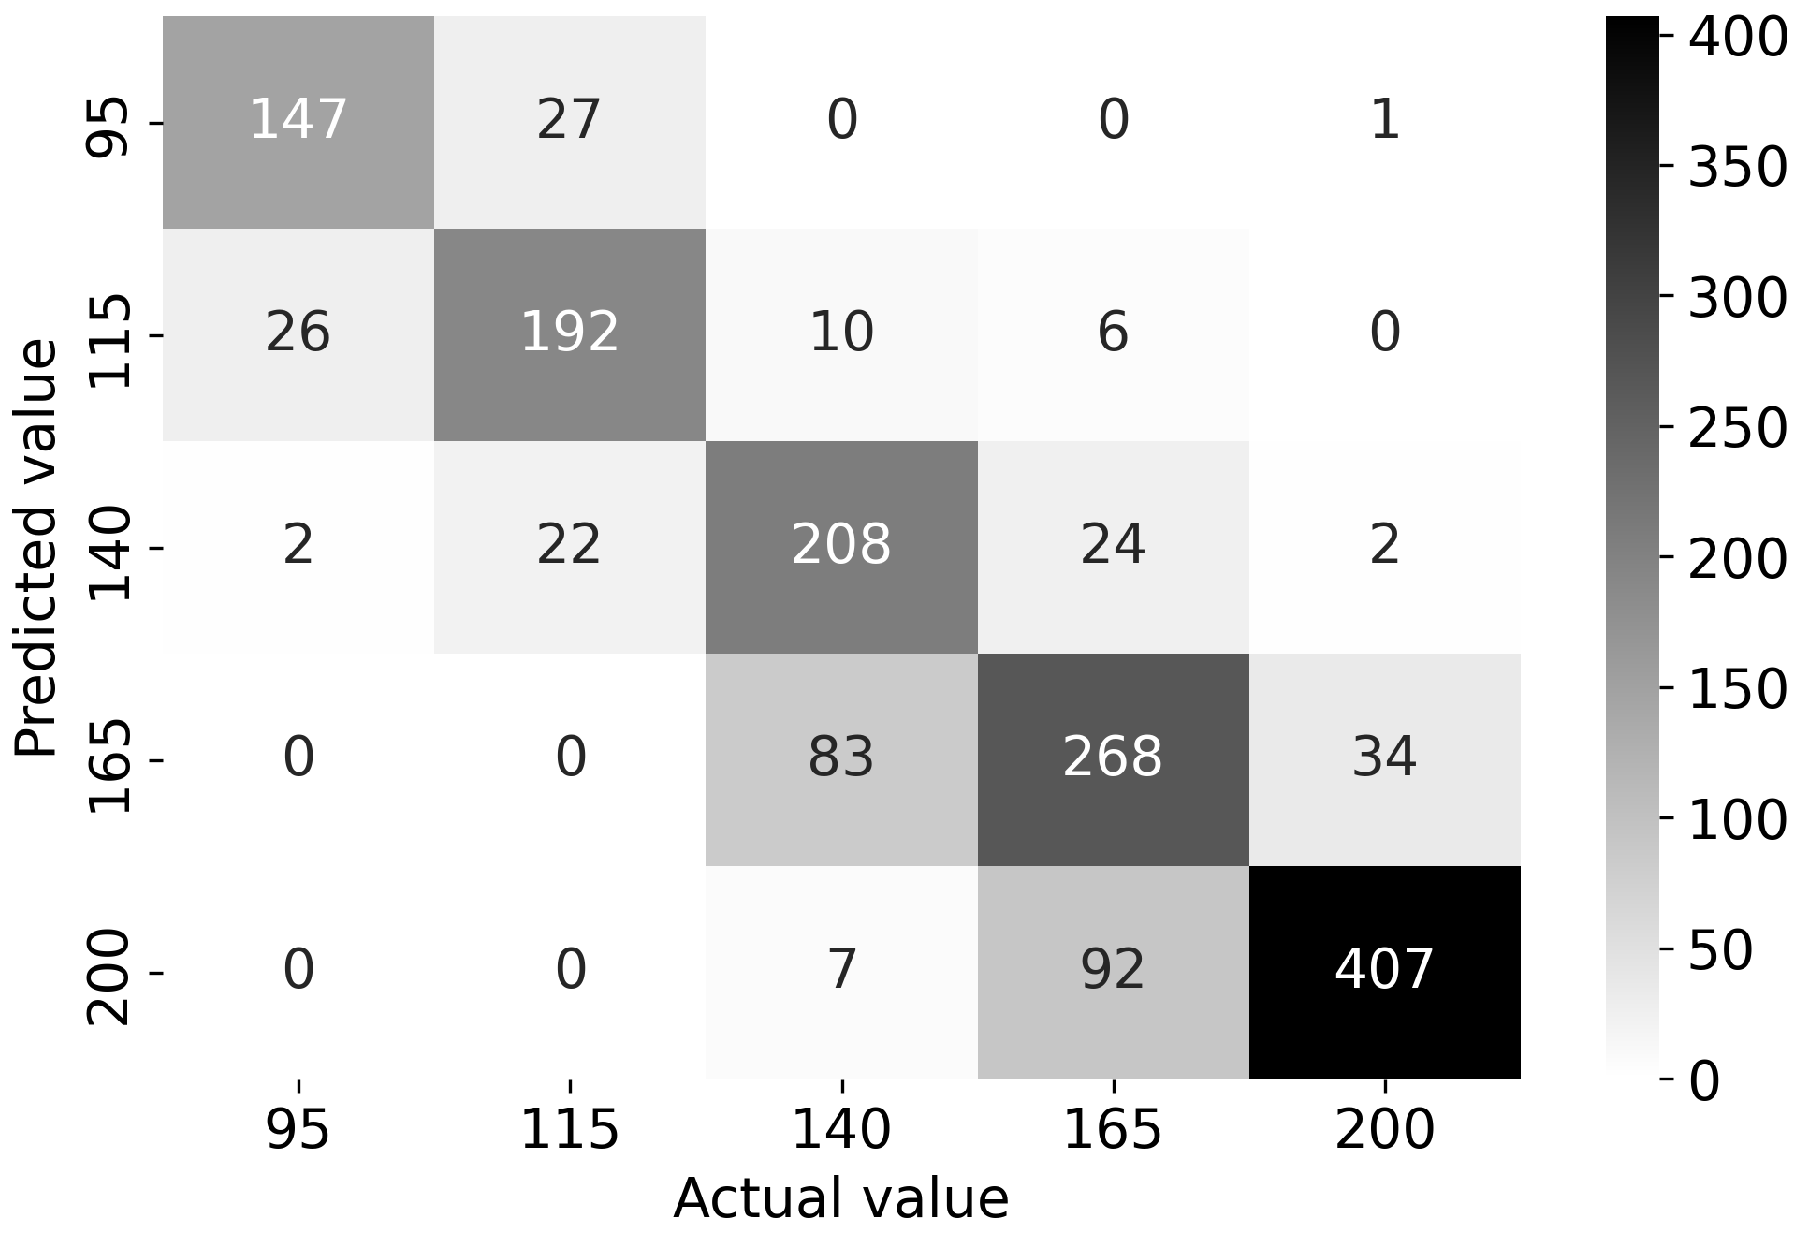
\includegraphics[width=0.90\linewidth]{2026_Citricos/figs/ConfusionMatrix_processes-14-00164-g013.png}    
\end{center}   
\end{column}

\end{columns}
 
\end{frame}

